% ****** Start of file apssamp.tex ******
%
%   This file is part of the APS files in the REVTeX 4.2 distribution.
%   Version 4.2a of REVTeX, December 2014
%
%   Copyright (c) 2014 The American Physical Society.
%
%   See the REVTeX 4 README file for restrictions and more information.
%
% TeX'ing this file requires that you have AMS-LaTeX 2.0 installed
% as well as the rest of the prerequisites for REVTeX 4.2
%
% See the REVTeX 4 README file
% It also requires running BibTeX. The commands are as follows:
%
%  1)  latex apssamp.tex
%  2)  bibtex apssamp
%  3)  latex apssamp.tex
%  4)  latex apssamp.tex
%
\documentclass[%
 reprint,
%superscriptaddress,
%groupedaddress,
%unsortedaddress,
%runinaddress,
%frontmatterverbose, 
%preprint,
%preprintnumbers,
%nofootinbib,
%nobibnotes,
%bibnotes,
 amsmath,amssymb,
 aps,
%pra,
%prb,
%rmp,
%prstab,
%prstper,
%floatfix,
]{revtex4-2}

\usepackage{tipa}
\usepackage{graphicx}% Include figure files
\usepackage{dcolumn}% Align table columns on decimal point
\usepackage{bm}% bold math
%\usepackage{hyperref}% add hypertext capabilities
%\usepackage[mathlines]{lineno}% Enable numbering of text and display math
%\linenumbers\relax % Commence numbering lines

%\usepackage[showframe,%Uncomment any one of the following lines to test 
%%scale=0.7, marginratio={1:1, 2:3}, ignoreall,% default settings
%%text={7in,10in},centering,
%%margin=1.5in,
%%total={6.5in,8.75in}, top=1.2in, left=0.9in, includefoot,
%%height=10in,a5paper,hmargin={3cm,0.8in},
%]{geometry}

\begin{document}

\preprint{APS/123-QED}

\title{2D Ising Model with MCMC:\\Group B}% Force line breaks with \\

\author{Blase Fencil}
 \email{@ucsd.edu}%Lines break automatically or can be forced with \\
\author{Zice Zhao}%
 \email{ziz084@ucsd.edu}
\author{Tristan Collis}
 \email{@ucsd.edu}

\date{\today}% It is always \today, today,
             %  but any date may be explicitly specified

\begin{abstract}
\begin{description}
\item[GitHub Repo]
\href{https://github.com/TristanCollis/Final-Ising-B/tree/main}{https://github.com/TristanCollis/Final-Ising-B/tree/main}
\end{description}
\end{abstract}

%\keywords{Suggested keywords}%Use showkeys class option if keyword
                              %display desired
\maketitle

%\tableofcontents

\section{\label{sec:level1}Introduction}

In this project, we use a MCMC method to simulate a 2D Ising spin lattice in varying magnetic fields and at varying temperatures. We explore parameters used to set up the simulation and see how certain starting conditions give rise to hysteresis and metastable states at low enough temperatures.

\subsection{\label{sec:level2}Ising Model}

For this project, we focus on the 2D Ising model, which consists of a lattice of spins $\{+1, -1\}$ and is often used to approximate ferromagnetic materials. The behavior of the system is described by an energy function $E(\sigma)$, where $\sigma$ represents the configuration of spins. The energy function is defined as:

\begin{equation}
E(\sigma) = -J\sum_{\langle ij \rangle} \sigma_i\sigma_j - B\sum_{i \in \Lambda}\sigma_i
\end{equation}

Here, $J$ denotes the coupling constant, $B$ represents the external magnetic field, and the terms $\sum_{\langle ij \rangle}$ and $\sum_{i \in \Lambda}$ represent summations over nearest neighbors and all spins, respectively. The symbol $\langle ij \rangle$ signifies pairs of adjacent lattice sites.

The first term $-J\sum_{\langle ij \rangle} \sigma_i\sigma_j$ captures the interaction energy between neighboring spins, where aligned neighbors have lower energy than opposing neighbors. The second term $-B\sum_{i \in \Lambda}\sigma_i$ represents the interaction of spins with the external magnetic field.

A significant consequence of this energy function is the tendency of the lattice to align with the external magnetic field at low temperatures, as spins converge towards the lowest energy state.

Furthermore, the magnetization $M(\sigma)$ of the system, defined as the average spin per site, is given by:

\begin{equation}
M(\sigma) = \frac{1}{|\Lambda|} \sum_{i \in \Lambda} \sigma_i
\end{equation}

Here, $|\Lambda|$ represents the total number of lattice sites.

Attach some snapshots of low temperature, negative magnetic field; low temperature, positive magnetic field.

\subsection{\label{sec:level2}Monte Carlo Markov Chain}  

Monte Carlo methods describe a broad class of algorithms that attempt to 
reduce operational complexity and computation time by replacing exhaustive 
computations with random ones. In this project, instead of computing the full dynamics of the system, which would be intractible, we pick a random cell in the lattice at each time step, and decide whether or not to flip it based on some probability dependent in the projected change in energy, and the predefined "temperature" of the system.  
  
A Markov Chain is a probabilistic state system in which each state has a defined probability to transition to each other state at every time step. These states are often visualized as nodes in a network, with eachdirected edge weighted according to the probability that the state will move along that edge from its initial to terminal nodes. In computing, this is more often computed as a transition matrix that encodes the same information.  
  
For our purposes, however, we do not necessarily know the full probability matrix, as the phase space for this problem is intractible to solve completely. Instead, we know the transition probability based on the state variables, and need to evolve the system in time based on that. This is where Monte Carlo Markov Chains help. By stepping around the phase space randomly, weighted according to known transition rules, we can more efficiently explore the phase space of the system in an approximate manner.

\section{\label{sec:level1}Results and Discussion}
\subsection{\label{sec:level2}Configuration and Burn-In}
We've developed an algorithm for determining the appropriate number of burn-in steps for a given Ising model simulation. The primary objective of this algorithm is computational efficiency.
If the absolute difference between these two values falls below the error threshold, we backtrack by 25\% of the array's length. We then compute the absolute difference of this value with \(h1\) and compare it against the error. If it exceeds the error, we move forward by 12.5\%; conversely, if it falls below the error, we backtrack by 12.5\%. It's worth noting that the percentage values we use for moving back and forth are based on the inverse powers of two, ensuring a geometrically decreasing step size. For instance, we move back by 50\% (\(1/2\)) of the array's length, then by 25\% (\(1/4\)), and subsequently by 12.5\% (\(1/8\)), and so forth. This geometric progression allows for a systematic exploration of the magnetization history, optimizing the search for the appropriate burn-in steps.

In the scenario where the first absolute difference yields a value greater than the error, we transition to a mean sampling method. Here, we randomly sample a subset of points (typically ranging from 5 to 20) from the magnetization history. Subsequently, we compute the mean of this sample and conduct a linear search from the beginning of the magnetization history. We continue this search until we locate a value below or above the mean, depending on whether the history is converging downwards or upwards.

\begin{figure}
    \centering
    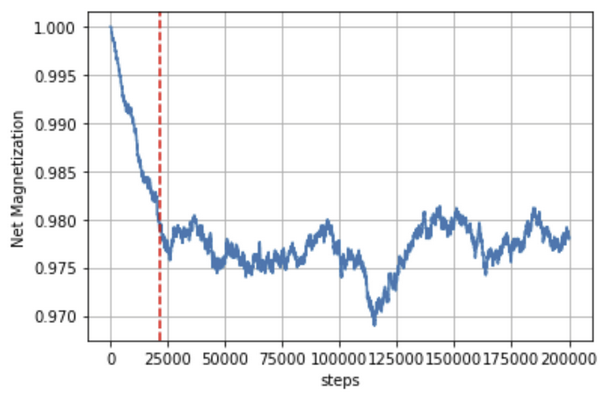
\includegraphics[width=1\linewidth]{burnin,upLattice.png}
    \caption{Burn-in, starting with all up spins}
    \label{fig:burnin,upLattice}
\end{figure}

\begin{figure}
    \centering
    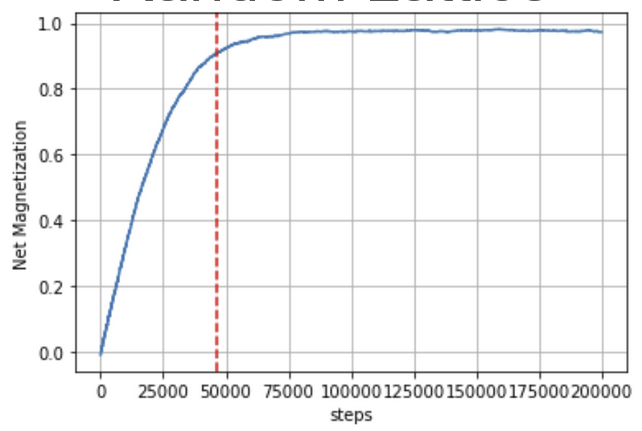
\includegraphics[width=1\linewidth]{burnin,randomLattice.png}
    \caption{Burn-in, starting with random spins}
    \label{fig:burnin,randomLattice}
\end{figure}

One notable advantage of this algorithm is its reliability in yielding results, albeit with a caveat. In instances where the magnetization history exhibits significant noise, the error-based method often fails, defaulting instead to mean sampling. However, it's worth noting that this may not always produce accurate results.

\subsection{\label{sec:level2}1D Scans of Magnetization vs Temperature}
When plotting magnetization vs temperature for constant magnetic field (figure \ref{fig:1dscans,fixedB}), we can observe that when the magnetic field (\(B\)) is zero, the net magnetization undergoes a rather sudden transition to an all-random state. Conversely, if there is any non-zero \(B\) field, the transition is much slower, but the net magnetization eventually converges to around zero, albeit at a higher temperature. These transitions to an all-random state represent a second-order phase transition of the material.

Plotting magnetization vs external field for fixed temperature (figure \ref{fig:1dscans,fixedT}), we observed a discontinuity at about \(B=0\) for low temperatures, corresponding to a first-order phase transition. For higher temperatures, we noticed that the net magnetization flattens out and converges to around zero, regardless of the magnetic field.

\begin{figure}
    \centering
    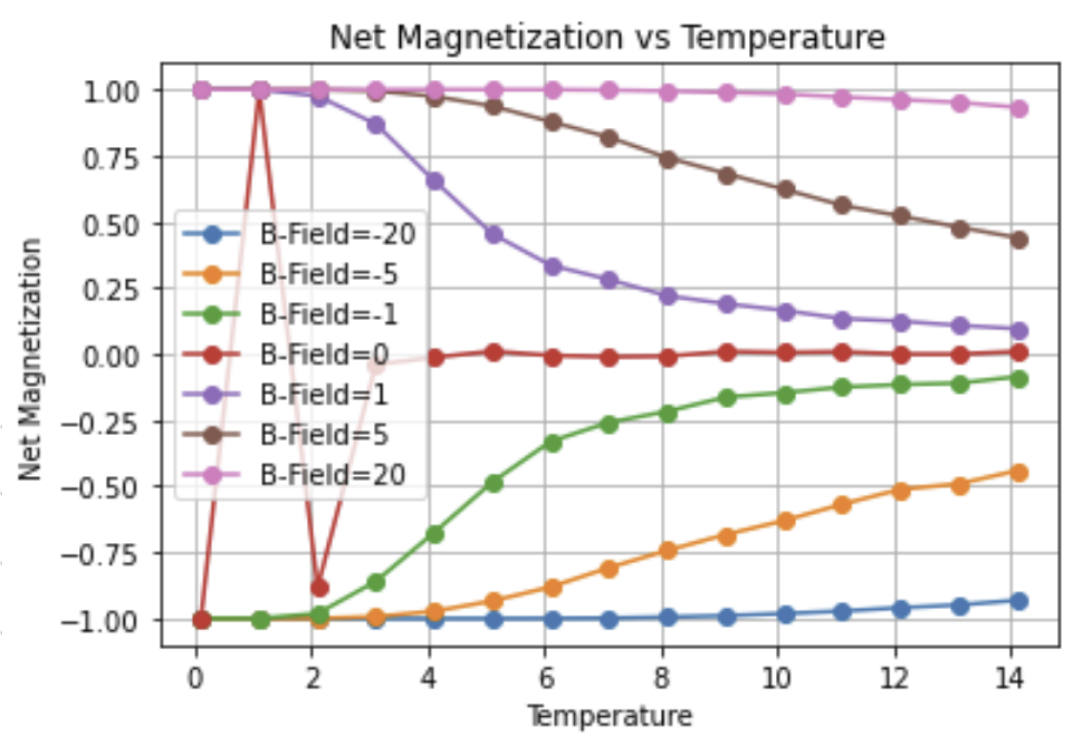
\includegraphics[width=1\linewidth]{1dscans,fixedB.png}
    \caption{M vs T for fixed B}
    \label{fig:1dscans,fixedB}
\end{figure}

\begin{figure}
    \centering
    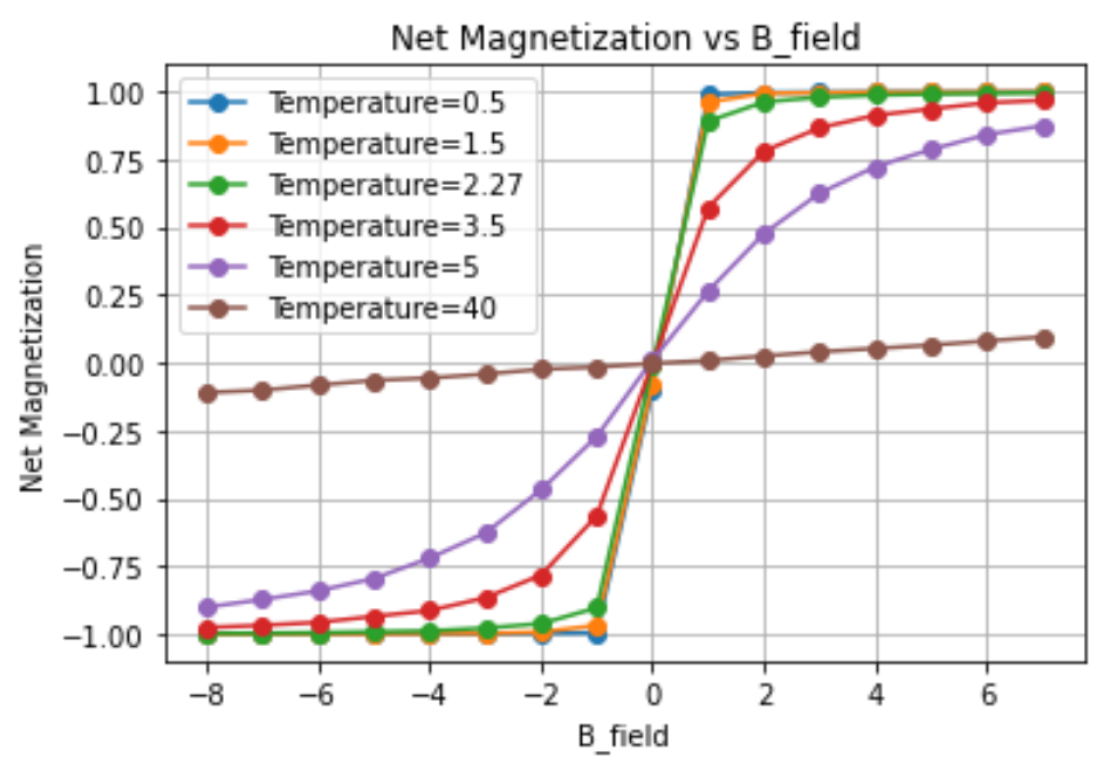
\includegraphics[width=1\linewidth]{1dscans,fixedT.png}
    \caption{M vs B for fixed T}
    \label{fig:1dscans,fixedT}
\end{figure}

\begin{figure}
    \centering
    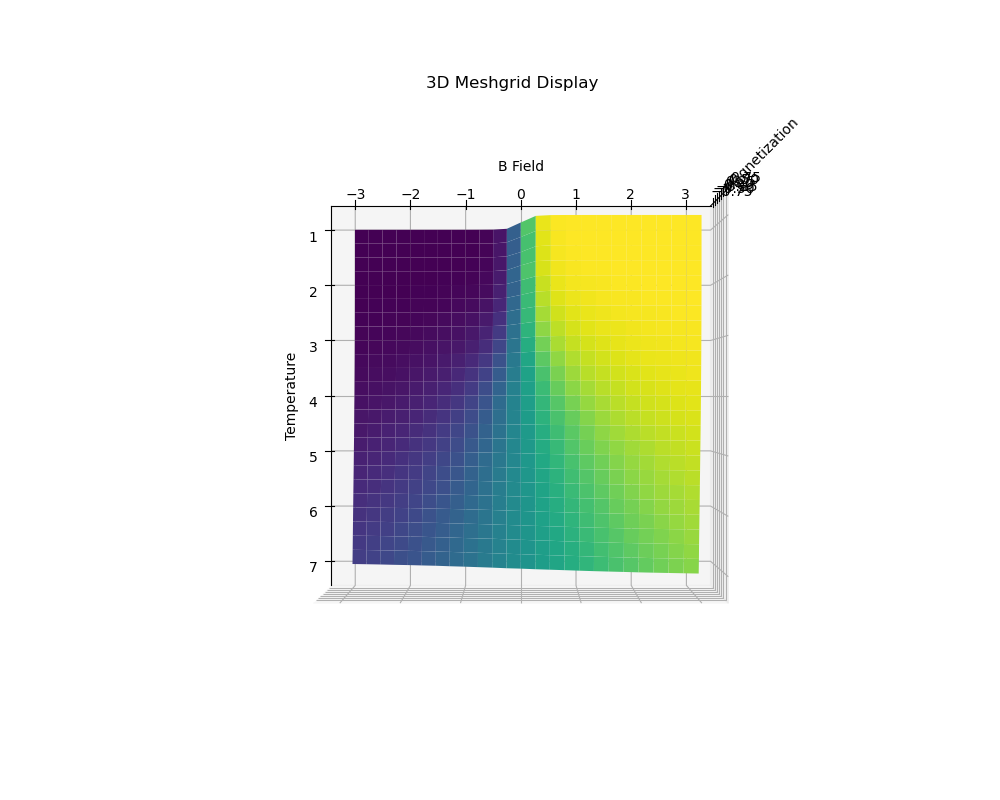
\includegraphics[width=1\linewidth]{graph_0.png}
    \caption{Phase Diagram}
    \label{fig:phase-diagram}
\end{figure}

\subsection{\label{sec:level2}Phase Diagram, Metastable States, and Hysteresis}

The inherent stability of aligned spins gives rise to metastable states - states that are local potential minima (resistant to perturbation and thus stable), but not global minima (i.e. not the least possible energy). Here, if a low-temperature lattice begins in an all-up or all-down state, it is able to resist an external field in the opposite direction for some time, before eventually becoming overpowered by a strong-enough field. 
This dependence upon the initial state is called hysteresis, and can give rise to lattices that have a sort of "memory" of their recent states. Systems that exhibit hysteresis are hard to solve analytically due to this dependence of the current state on prior states.
We have graphed some of these hysteresis curves, where the phase transition from down to up or up to down spin depends on which way the aligned spins began in (figures \ref{fig:hysteresis_spin_down} and \ref{fig:hysteresis_spin_up}).

\begin{figure}
    \centering
    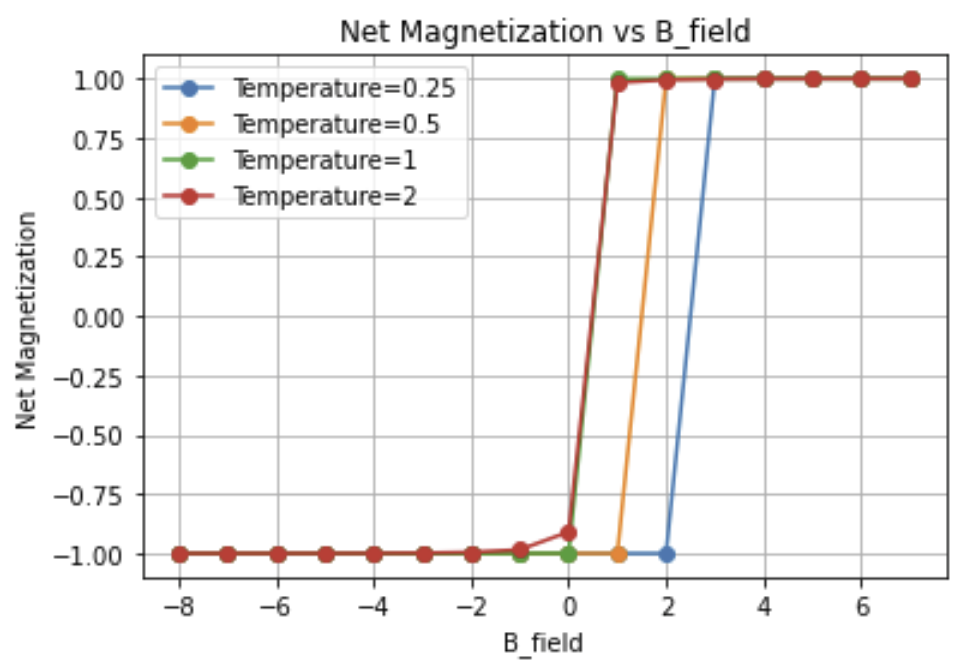
\includegraphics[width=1\linewidth]{hysteresis_spin_down.png}
    \caption{Enter Caption}
    \label{fig:hysteresis_spin_down}
\end{figure}

\begin{figure}
    \centering
    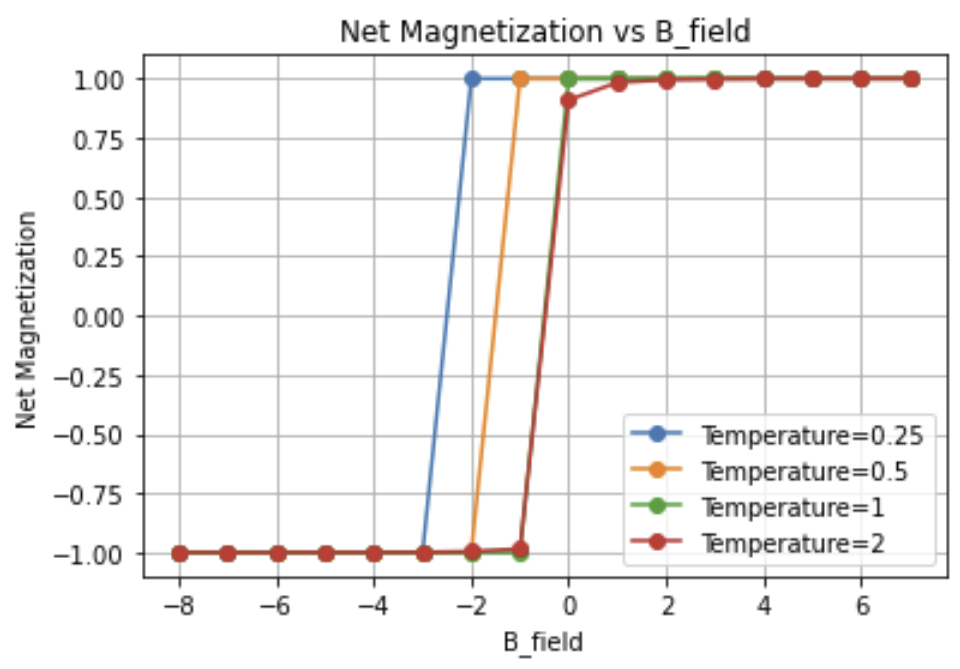
\includegraphics[width=1\linewidth]{hysteresis_spin_up.png}
    \caption{Enter Caption}
    \label{fig:hysteresis_spin_up}
\end{figure}

\section{\label{sec:level1}Profiling and Optimization}
To make the code run in a reasonable amount of time, we used a combination of high code separation, Numba, and Scalene.
In general, to make the most use out of the tools we had, we used a functional style of programming, and separated code functionality as far as we could, trying as much as possible to ensure each function had as few responsibilities as possible (preferably exactly 1). This way, when we optimized, we could fast-track development by limiting Numba applications only the code most critical to performance, reducing the need to untangle the strict typing and compilation requirements to get Numba working on a larger scale. It also helped us to profile code, as while the tool we used, Scalene, can profile individual lines of code, it is much better at profiling entire functions.
Numba is a set of C libraries with a front-end accessible via Python. This allows developers to use highly performant C code from within much easier-to-use Python. It works best when breaking down loops and iterations, as well as large matrix operations, which Python struggles to do at speed by itself.
Lastly, we used Scalene, a profiling tool that tracks time spent per line and per function in the code, including the proportions of time spent by the processor running in Python, native bytecode, and C. It also tracks memory and GPU usage.
With the combination of these three, we were able to track down the fact that our performance bottleneck lay in the $\Delta E$ calculation during simulation steps when determining whether or not to flip a cell's spin. Figure \ref{fig:Scalene-Screenshot} is a screen capture of our code's performance running a low-resolution pass.

\begin{figure}
    \centering
    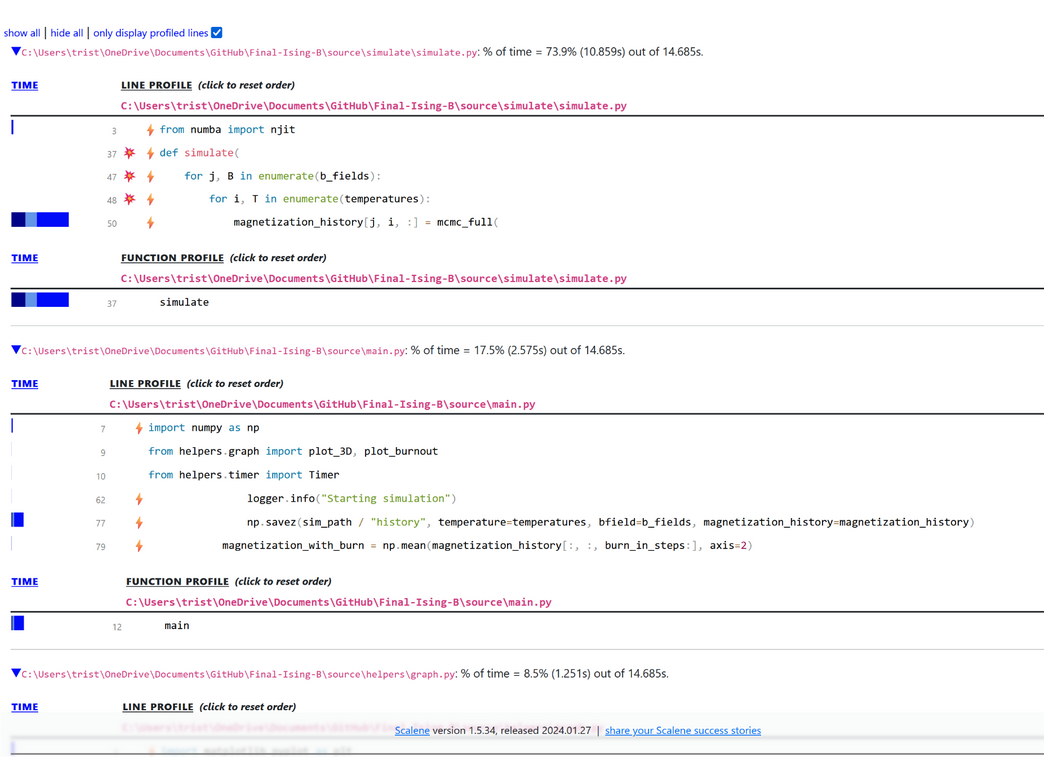
\includegraphics[width=1\linewidth]{Scalene-Screenshot.png}
    \caption{Scalene profile of our simulation}
    \label{fig:Scalene-Screenshot}
\end{figure}


 

\end{document}
%
% ****** End of file apssamp.tex ******
